\section{Ring Imaging Cherenkov Detectors (RICH)}
\subsection*{Cherenkov Radiation}
Charged particles traversing through a medium at a speed greater than the speed of light in the same medium emit electromagnetic radiation known as Cherenkov radiation. The angle at which the radiation is emitted relative to the direction of the particle (Cherenkov angle, $\theta_C$) is constant given the speed of the particle and the refractive index of the medium are also constant. The relationship between the speed of the particle ($\beta = |\vec{v}|/c$), refractive index of the medium ($n$) and the Cherenkov angle ($\theta_C$) is described by the equation,

\begin{equation}
	\cos{\theta_C} = \frac{1}{n\beta}\\
	\label{equation: Cherenkov radiation}
\end{equation}

The speed of the particle, $\beta$ can be expressed in terms of its mass $m$ and momentum $\vec{p}$, the equation for the Cherenkov angle in these terms is then,

\begin{equation}
	\cos{\theta_C} = \frac{1}{n}\sqrt{1 + \frac{m^2}{p^2}}
	\label{equation: Cherenkov angle in terms of mass and momentum}
\end{equation}

where $\beta=\frac{|\vec{p}|}{E} = \frac{|\vec{p}|}{\sqrt{p^2 + m^2}} = \frac{1}{\sqrt{1 + m^2/p^2}}$. For a charged particle emitting Cherenkov radiation, measurements of the Cherenkov angle of its emitted photons together with its momentum information (e.g. using information from tracking systems) and the above relationship allows the calculation of its mass and hence particle type (particle and anti-particles can be distinguished by their charge, e.g from the direction of bend when passing through a magnetic field). Measurements of the Cherenkov angle in the LHCb detector are achieved through its RICH system. 

%$|\vec{p}|\sqrt{(n^2 cos^2(\theta_C) - 1)}$

%\begin{eqnarray}
%	\beta&=&\frac{|\vec{p}|}{E}
%	= \frac{|\vec{p}|}{\sqrt{\vec{p}^2 + m^2}}
%	= \frac{1}{\sqrt{1 + m^2/\vec{p}^2}}
%	= \frac{\gamma m |\vec{v}|}{\gamma m} \,\,\,\,\,\,\,\,\,\,\,\,\,\,\,\,\,\,\,\, c = 1
%\end{eqnarray}

%It detects charged particles via their Cherenkov radiation emitted when traversing a medium of refractive index $n$ faster than the speed of light in the same medium
\subsection*{Requirements of the RICH detector}
%The RICH system is a key component in the LHCb particle identification system; it is 
The RICH is designed to provide excellent discrimination between charged hadrons, in particular, pions, kaons, and protons (though identification of charged leptons is also possible). This allows the discrimination between different hadronic decays, in particular, processes with similar topologies but different final states e.g. $B^0 \rightarrow h^+h^-$ \cite{JHEP10(2012)037} (figure \ref{fig: inv_mass_b_to_hh}), $B_c^+ \rightarrow J/\psi \pi^+\pi^-\pi^+$ \cite{PhysRevLett.108.251802},  $B^+ \rightarrow DK^+$ \cite{Aaij2012203}, $B^0\rightarrow K^{*0}\gamma$ \cite{PhysRevD.85.112013} and $B_s^0 \rightarrow K^\pm \pi^\mp$ \cite{PhysRevLett.108.201601}.

\begin{figure}[htbp]
	\begin{center}
		\begin{subfigure}[b]{0.49\textwidth}
			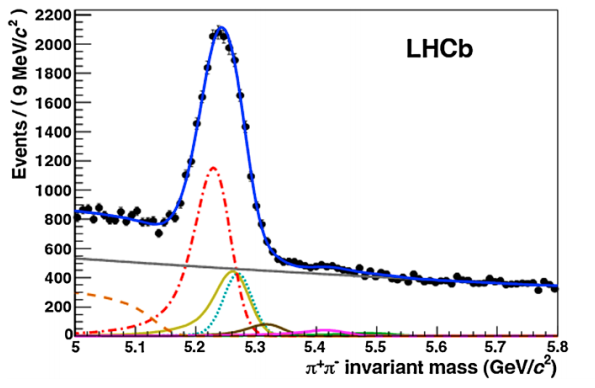
\includegraphics[width=\textwidth]{./Chapters/detector/rich/inv_mass_b_to_hh_no_rich.png}
			\caption{Without RICH information}
			\label{fig: inv_mass_b_to_hh_no_rich.png}
		\end{subfigure}
		\begin{subfigure}[b]{0.49\textwidth}
			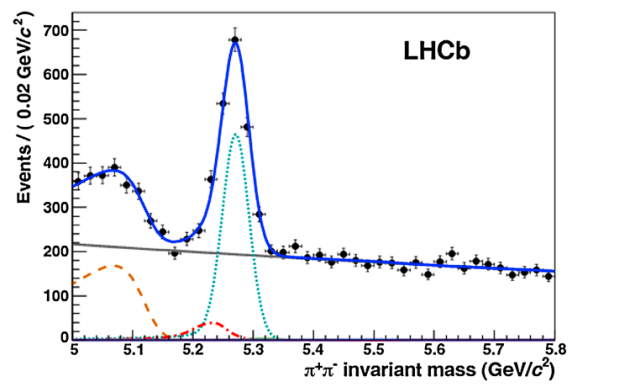
\includegraphics[width=\textwidth]{./Chapters/detector/rich/inv_mass_b_to_hh_with_rich.png}
			\caption{With RICH information}
			\label{fig: inv_mass_b_to_hh_with_rich.png}
		\end{subfigure}
		\caption{Invariant mass distribution of $B\rightarrow h^+h^-$ decays before (A) and after (B) inclusion of RICH information to isolate the signal decay, $B^0 \rightarrow \pi^+\pi-$ (teal dashed). The background processes are $B^0\rightarrow K\pi$ (red dashed-dotted), $B^0 \rightarrow$ 3-body (orange dashed), $B_s \rightarrow KK$ (yellow), $B_s \rightarrow K\pi$ (brown) $\Lambda_b \rightarrow pK$ (purple) and $\Lambda_b \rightarrow p\pi$~(green). There is also a contribution from combinatorial background (grey).}
		\label{fig: inv_mass_b_to_hh}
	\end{center}
\end{figure}

In addition to the discrimination between exclusive decay processes, information from the RICH detector is also used to make more general decisions on whether an event is of interest e.g. identification of events with at least one $\phi$ particle (which are present in many decay modes of interest). These decisions require significantly less CPU processing than exclusive event selection such that they are well suited to the strict time constraints of the trigger system, see section \ref{section: trigger}.

In a addition to direct processes (where the charged hadron identified is part of the processes being investigated) the particle identification also provides a method of flavour tagging in measurements of CP asymmetries or particle anti-particle oscillations. Such particles which are used to tag events typically have lower transverse momenta than particles from the decay of heavy B mesons. In order to satisfy the requirements stated previously the RICH must maintain good performance over a large range of momenta (2-100 GeV/c \cite{JHEP10(2012)037}).

\subsection*{Detector Description}

The RICH system consists of two RICH detectors, RICH1 and RICH2 \cite{Amato:494263}. RICH1 is positioned directly downstream of the Vertex Locator (VELO) and upstream of the magnet; it is attached directly to the VELO exit window. RICH2 is positioned downstream of the magnet and Tracking stations (T1, T2 and T3). They are approximately 1 m and 10 m downstream of the nominal interaction interaction point respectively (see figure \ref{fig: lhcb_schematic}), cover an angular acceptance of $\pm(25-300)$ [$\pm(15-120)$] mrad and momentum range of $2-40$ [$15-100$] GeV/c see figure \ref{fig: rich_angular_and_momentum_coverage}.

In order for Cherenkov radiation to occur a medium with a refractive index $n>1$ is required. The RICH system employs three different mediums (in the context of RICH detectors these are more commonly referred to as radiators) in order to cover the desired momentum range, see figure \ref{fig: radiators}. RICH1 contains both an aerogel and $\mathrm{C}_4\mathrm{F}_{10}$ gas whilst RICH2 contains only $\mathrm{CF}_4$ gas. The refractive indices of these are 1.03, 1.0014 and 1.0005 (at $0^\circ$, $101$ kPa and for photons with a wavelength of 400 nm) respectively.

\begin{figure}[htbp]
	\begin{center}
		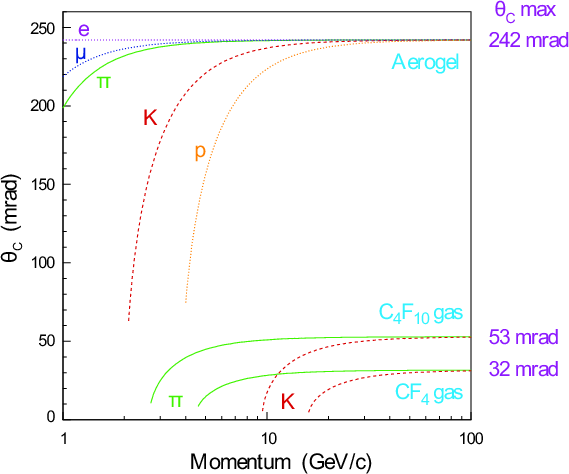
\includegraphics[width=0.6\textwidth]{./Chapters/detector/rich/radiators.png}
		\caption{Cherenkov angle $\theta_C$ as a function of particle momentum, particle type and radiator type.}
		\label{fig: radiators}
	\end{center}
\end{figure}


\begin{figure}[htbp]
	\begin{center}
		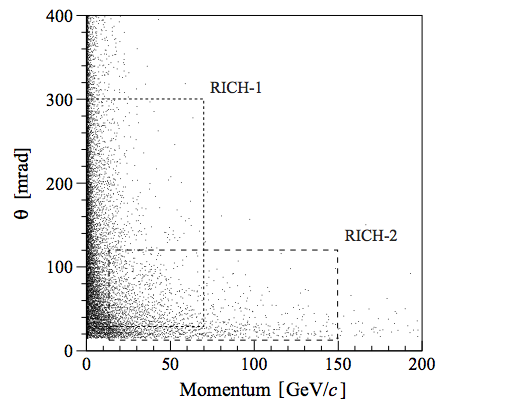
\includegraphics[width=0.6\textwidth]{./Chapters/detector/rich/rich_angular_and_momentum_coverage.png}
		\caption{Polar angle $\theta$ and momentum $p$ distribution of the tracks in simulated $B^0\rightarrow \pi^+\pi^-$ decays. The angular coverage and momentum range or the RICH detectors are shown by the regions contained in the dotted lines.}
		\label{fig: rich_angular_and_momentum_coverage}
	\end{center}
\end{figure}

Cherenkov photons emitted by charged particles passing through the radiators in the RICH detectors are emitted at a constant angle relative to the direction of the charged particle, this is referred to as the Cherenkov angle, $\theta_C$. Focusing these photons onto a plane with a parabolic mirror results in rings of photons in which the Cherenkov angle can be calculated from the radius. Both RICH detectors employ similar mirror systems; using a spherical mirror to focus the rings and a plane mirror to reflect the rings onto a plane of photon detectors, see figure \ref{fig: rich_system_schematic}. The purpose of the plane mirrors is to direct photons away from the detector where space limitations, radiation and strong magnetic fields create an undesirable environment for the operation of photon detectors. Each of the mirrors are composed of segments, see table \ref{tab: mirror_segmentation} and figure \ref{fig: mirror_segmentation_rich2}

\begin{figure}[htbp]
	\begin{center}
		\begin{subfigure}[b]{0.49\textwidth}
			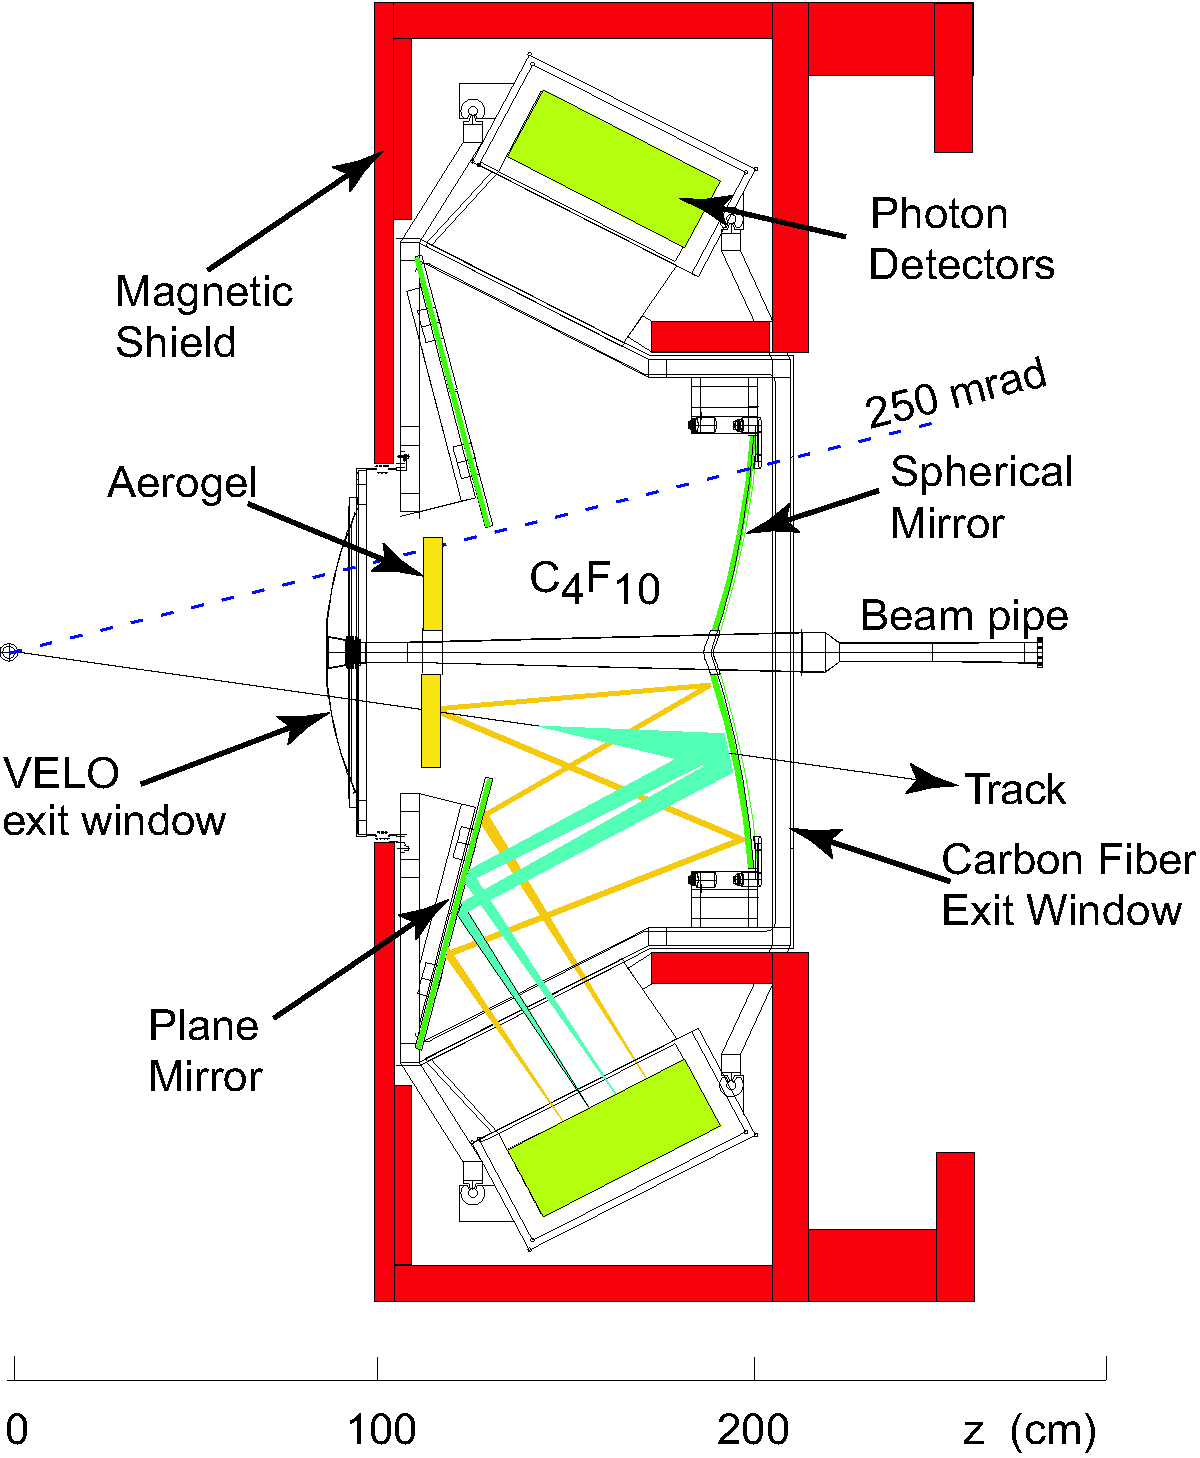
\includegraphics[width=\textwidth]{Chapters/detector/rich/rich1_schematic.png}
			\caption{RICH1, side view}
			\label{fig: rich1_schematic}
		\end{subfigure}
		\begin{subfigure}[b]{0.49\textwidth}
			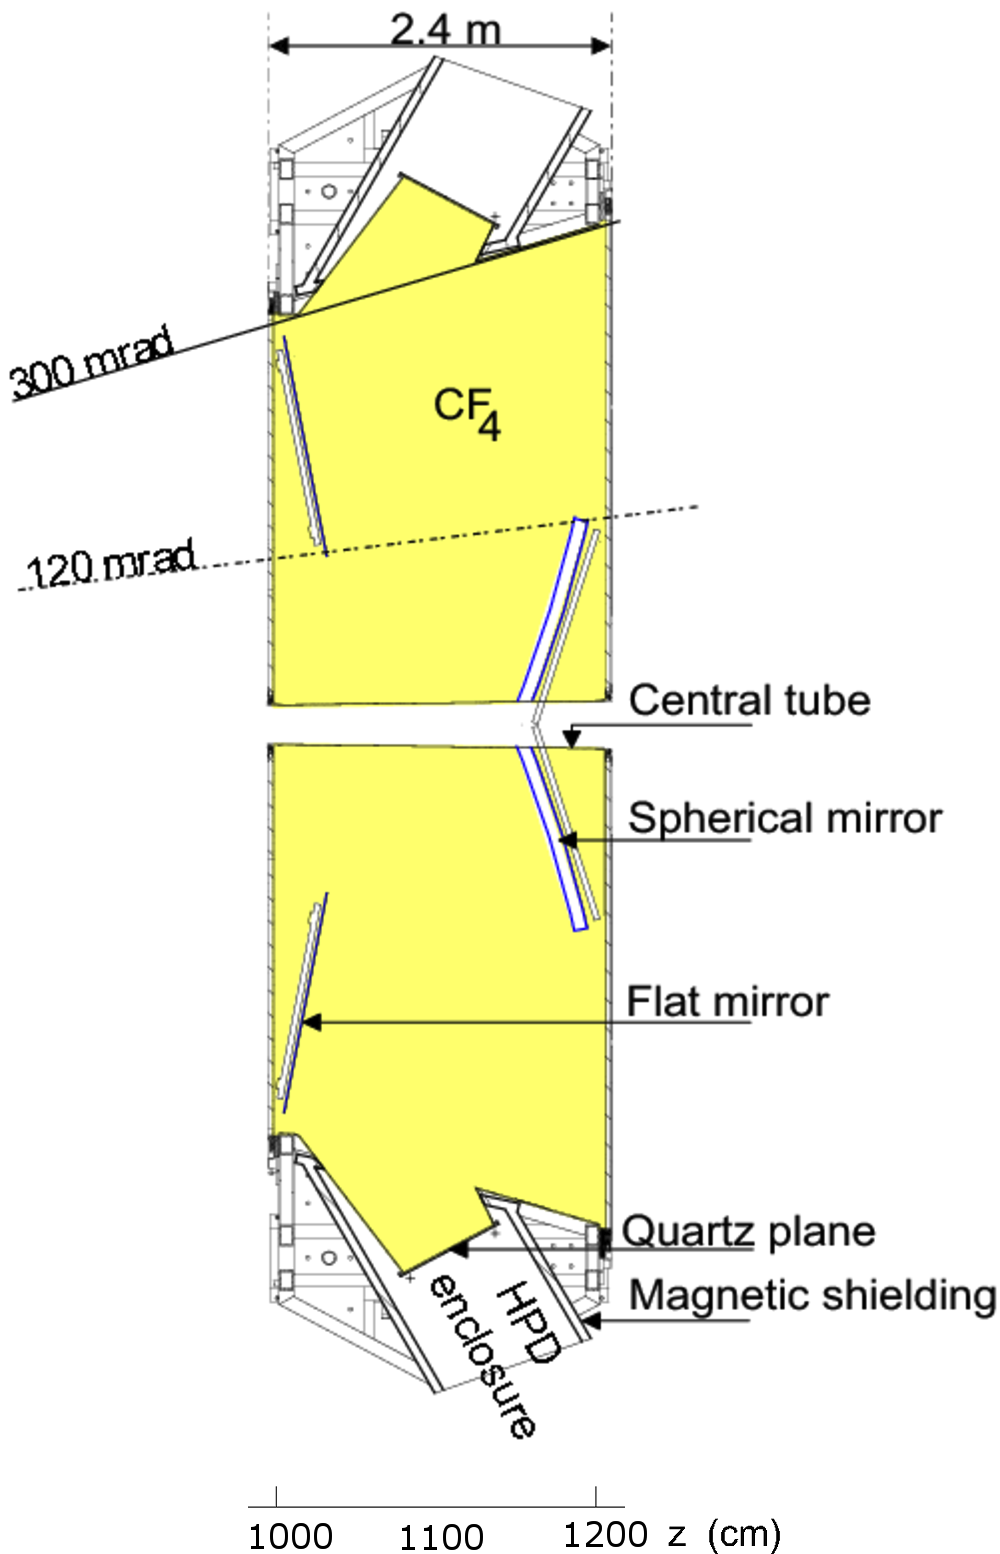
\includegraphics[width=\textwidth]{Chapters/detector/rich/rich2_schematic.png}
			\caption{RICH2, top view}
			\label{fig: rich2_schematic}
		\end{subfigure}
		\caption{Schematic of the RICH detectors, RICH1 (A) and RICH2 (B). The beam pipe runs left to right in both images.}
		\label{fig: rich_system_schematic}
	\end{center}
\end{figure}

\begin{table}[htdp]
	\caption{Spherical and plane mirror segmentation scheme in the RICH detectors.}
	\begin{center}
		\begin{tabular}{|c|c|c|}
			\hline
			& Spherical Mirror Segments & Plane Mirror Segments \\ \hline
			RICH1 & 4 & 16 \\ \hline
			RICH2 & 56 & 40 \\ \hline
		\end{tabular}
	\end{center}
	\label{tab: mirror_segmentation}
\end{table}%

\begin{figure}[htbp]
	\begin{center}
		\begin{subfigure}[b]{0.35\textwidth}
			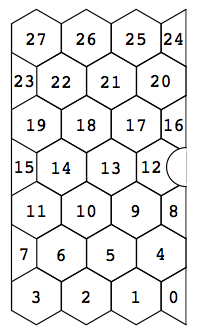
\includegraphics[width=\textwidth]{Chapters/detector/rich/mirror_segmentation_rich2_spherical.png}		
			\caption{}
			\label{}
		\end{subfigure}
		\begin{subfigure}[b]{0.35\textwidth}
			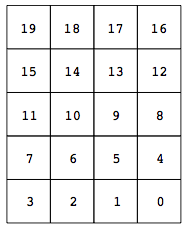
\includegraphics[width=\textwidth]{Chapters/detector/rich/mirror_segmentation_rich2_plane.png}
			\caption{}
			\label{}
		\end{subfigure}
		\caption{Schematic of the spherical (A) and plane (B) mirror segments for the left half of the RICH2 detector. Also shown is the numbering scheme used}
		\label{fig: mirror_segmentation_rich2}
	\end{center}
\end{figure}

The photon detector planes are arrays containing Hybrid Photon detectors (HPDs). There are two planes per RICH detector; Up and Down boxes in RICH1 (containing additional magnetic shields due to their proximity to the magnet) and the Left and Right boxes in RICH2, see figure \ref{fig: rich_system_schematic}. There are a total of 484 HPDs in the RICH system with 196 of them in the RICH1 detector and 288 in the RICH2 detector. 

The entrance to the HPDs consists of a quartz entrance window with a photocathode layer painted on the inner side of the window (see figure \ref{fig: hpd_schematic}). Photons incident on an HPD stimulate the emission of electrons into a vacuumed cavity inside the HPD via the photocathode layer. These electrons are then accelerated by an electric field across a potential difference of 16 kV onto a 32 x 32 silicon chip array with a pixel size of 2.5 mm x 2.5 mm. The chip records the position of the electron which is used to reconstruct the track of the photon from its emission point in the radiator to photocathode layer on the HPD entrance window. The Cherenkov angle can then be calculated by coupling the photon to its corresponding charged particle and calculating the relative angle between the two.

\begin{figure}[htbp]
	\begin{center}
		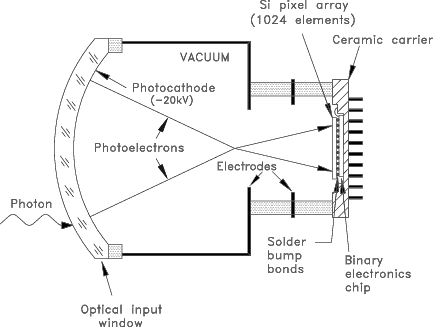
\includegraphics[width=0.6\textwidth]{./Chapters/detector/rich/hpd_schematic.png}
		\caption{Schematic diagram of a Hybrid Photon Detector (HPD)}
		\label{fig: hpd_schematic}
	\end{center}

\end{figure}

\subsubsection*{Performance - Cherenkov Angle Resolution}
For a medium with refractive index $n$ and where $|\vec{p}| >> m$ the Cherenkov angle becomes \emph{saturated} such that for all particle types the Cherenkov equation (equation \ref{equation: Cherenkov angle in terms of mass and momentum}) can be expressed as,

\begin{equation}
	\cos{\theta_C^{max}} = \frac{1}{n}
	\label{equation: saturated Cherenkov radiation}
\end{equation}

such that the Cherenkov angle for all particle types converge,

\begin{equation}
	\theta_C^{max}(\pi) = \theta_C^{max}(K) = \theta_C^{max}(p)
\end{equation}

\emph{Saturation} of the Cherenkov angle in the LHCb RICH detector can be seen in the high momentum regions of figure \ref{fig: radiators}. The saturation Cherenkov angles are 242 mrad, 53 mrad and 32 mrad for the Aeorogel $\mathrm{C}_4\mathrm{F}_{10}$ and $\mathrm{CF}_4$ radiators respectively. The alignment of the RICH detector can then be tested by plotting the distribution of the difference between the measured Cherenkov angle and the saturated Cherenkov angle, $\Delta\theta_C = \theta_C$ - $\theta_C^{max}$ for photons emitted from saturated tracks.%; %if the detector is perfectly aligned then this distribution will be described by a delta function, $\delta(\Delta\theta)$.

%\subsubsection*{Performance - Particle Identification} edit